\subsection{Classification Metrics}
\subsubsection{Confusion Matrix}
Perhaps the place to start when evaluating classification models is the confusion matrix. Figure \ref{fig:confusion} shows an excellent figure from Wikipedia displaying what this matrix looks like.

 \begin{figure}[h] \label{fig:confusion}
\caption{Plot from Wiki showing confusion matrix}
\centering
 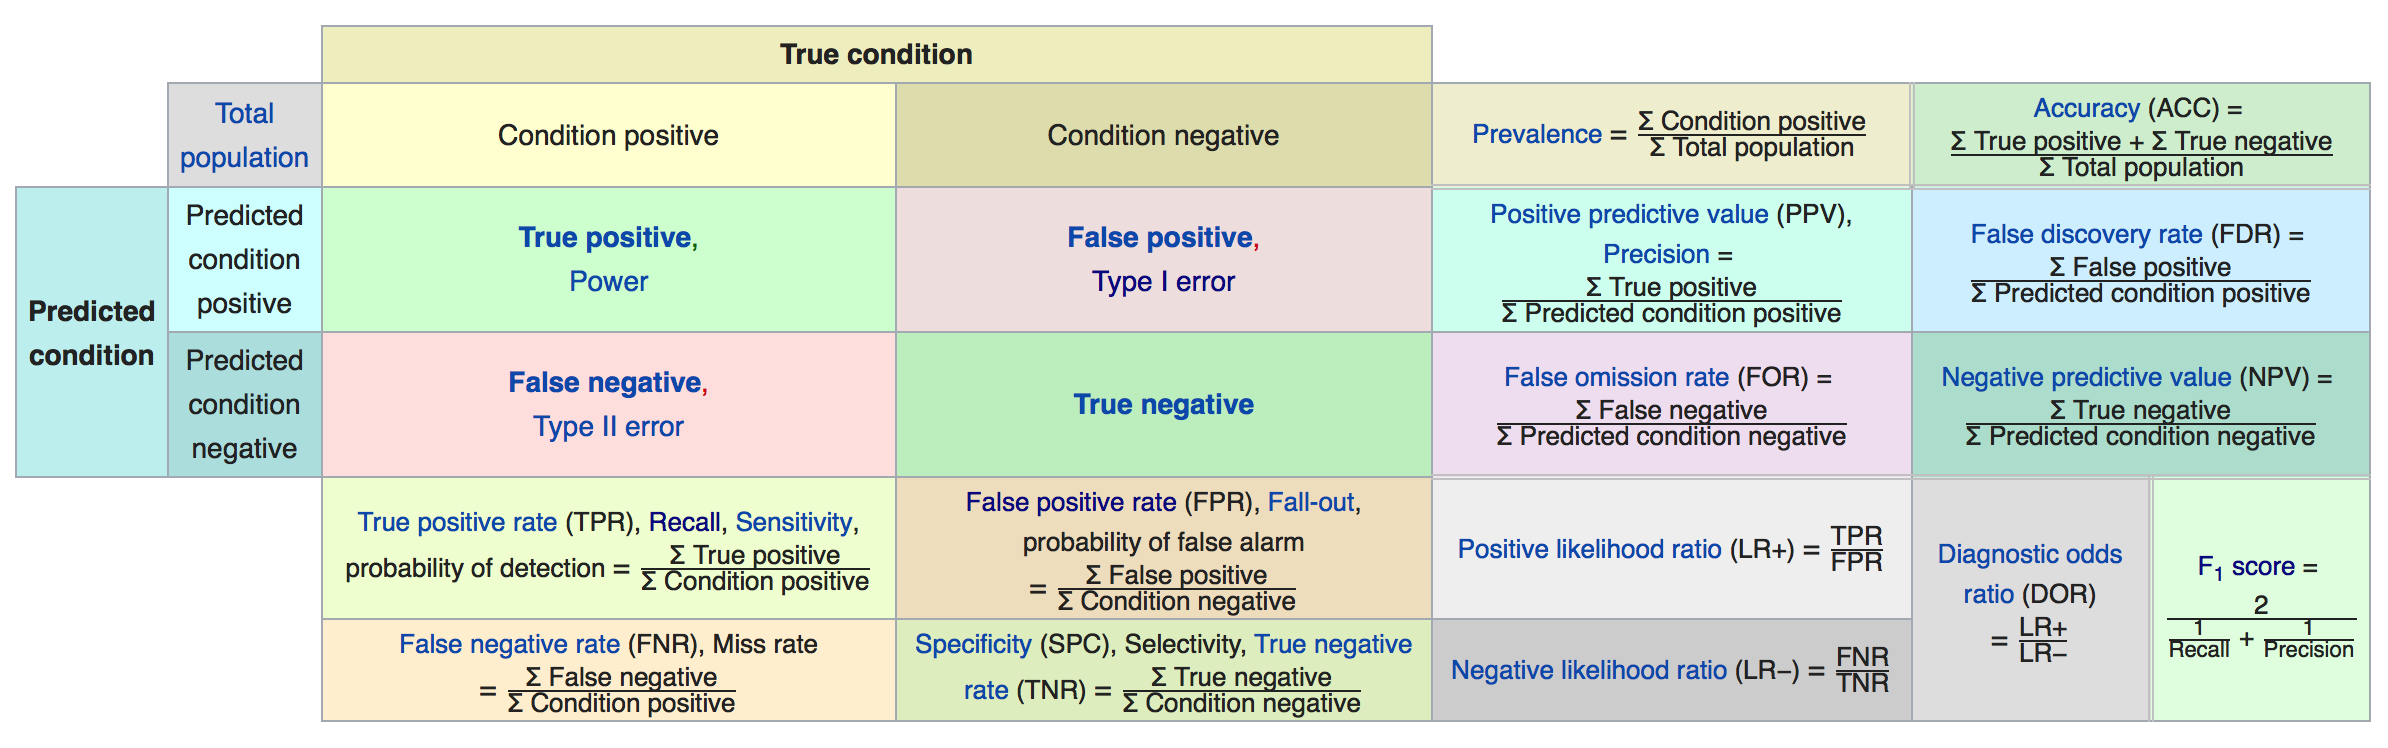
\includegraphics[scale=.4]{confusion_matrix.png}
 \end{figure}
 
 The columns represent the true class (positive or negative) and the rows represent the predicted class (positive or negative). The cross-intersection of these predictions and truth create four areas: \emph{true positives} (number of instances that are predicted positive that actually are positive), \emph{false positives} (number of instances that are predicted positive that are actually negative), \emph{false negatives} (number of instances that are predicted negative that are actually positive) and \emph{true negatives} (number of instances that are predicted negative that actually are negative).
 
 In the Wiki figure there are three other terms in the 2x2 confusion matrix namely power, Type 1 error, and Type 2 error. TODO
 
 